% WSCG sample document 
%
% based on Gabriel Zachmann's sample
% http://zach.in.tu-clausthal.de/latex/
%
% modified Apr 2012 to match WSCG Word template
%
\documentclass[twoside,twocolumn,10pt]{article}
%\documentclass[twoside,twocolumn,draft]{article}

%  for debugging
%\tracingall%\tracingonline=0
%\tracingparagraphs
%\tracingpages


%%%%%%%%%%%%%%%%%%%%%%%%%%%%%%%%%%%%%%%%%%%%%%%%%%%%%%%%%%%%%%%%%%%%%%%%%%%%%
%                             Packages

\usepackage{wscg}           % includes a number of other packages (e.g., myalgorithm)
\RequirePackage{ifpdf}
\ifpdf
 \RequirePackage[pdftex]{graphicx}
 \RequirePackage[pdftex]{color}
\else
 \RequirePackage[dvips,draft]{graphicx}
 \RequirePackage[dvips]{color}
\fi
%\usepackage[german,english]{babel}     % default = english
%\usepackage{mypicture}      % loads graphicx.sty, color.sty, eepic.sty
%\usepackage{array}          % better tabular's & arrays, plus math tabular's
%\usepackage{tabularx}      % for selfadjusting p-columns
%\setlength{\extrarowheight}{1ex}   % additional space between rows
%\usepackage{booktabs}      % typographically much better
%\usepackage{mdwlist}        % for compacted lists, and more versatile lists
%\usepackage[intlimits]{amsmath} % more math stuff, see texdoc amsldoc
%\usepackage{mymath}         % own commands, loads amssymb & array.sty
%\usepackage{hyphenat}      % hyphenatable -, /, etc.
%\usepackage{theorem}
%\usepackage[sort&compress]{natbib}% better \cite commands, more flexible
%\usepackage[sort&compress,super]{natbib} % better \cite commands, more flexible
%\newcommand{\citenumfont}[1]{\textit{#1}}


\usepackage{nopageno}       % no page numbers at all; uncomment for final version

\usepackage{subfig}
\usepackage{graphicx}
%%%%%%%%%%%%%%%%%%%%%%%%%%%%%%%%%%%%%%%%%%%%%%%%%%%%%%%%%%%%%%%%%%%%%%%%%%%%%
%                                Title

\title{Automatic morphology: Application on biological images}

\author{
\parbox{0.25\textwidth}{\centering
LE Van Linh\\[1mm]
ITDLU\\
Dalat University\\
Vietnam\\
linhlv@dlu.edu.vn
}
\hspace{0.05\textwidth}
\parbox{0.25\textwidth}{\centering
BEURTON-AIMAR Marie\\[1mm]
LaBRI-CNRS 5800\\
Bordeaux University\\
33400 Talence-F\\
beurton@labri.fr
}
\hspace{0.05\textwidth}
\parbox{0.25\textwidth}{\centering
PARISEY Nicolas\\[1mm]
IGEPP\\
INRA 1349\\
35653 Le Rheu-F\\
nparisey@rennes.inra.fr
}
}

%%%%%%%%%%%%%%%%%%%%%%%%%%%%%%%%%%%%%%%%%%%%%%%%%%%%%%%%%%%%%%%%%%%%%%%%%%%%%
%                          Hyperref


% no hyperlinks
\usepackage{url}
\urlstyle{tt}

% Donald Arsenau's fix for missing kerning of "//" and ":/"
\makeatletter
\def\Uslash{\mathbin{\mathchar`\/}\@ifnextchar{/}{\kern-.15em}{}}
\g@addto@macro\UrlSpecials{\do \/ {\Uslash}}
\def\Ucolon{\mathbin{\mathchar`:}\@ifnextchar{/}{\kern-.1em}{}}
\g@addto@macro\UrlSpecials{\do : {\Ucolon}}
\makeatother





%%%%%%%%%%%%%%%%%%%%%%%%%%%%%%%%%%%%%%%%%%%%%%%%%%%%%%%%%%%%%%%%%%%%%%%%%%%%%
%                              My Commands


%\DeclareMathOperator{\sgn}{sgn}

%\theorembodyfont{\upshape}
%\theoremstyle{break}
%\theoremheaderfont{\bfseries\normalsize}

%\newtheorem{lem}{Lemma}
%\newtheorem{defn}{Definition}



%%%%%%%%%%%%%%%%%%%%%%%%%%%%%%%%%%%%%%%%%%%%%%%%%%%%%%%%%%%%%%%%%%%%%%%%%%%%%
%                                Document


\begin{document}

\twocolumn[{\csname @twocolumnfalse\endcsname

\maketitle  % full width title


\begin{abstract}
\noindent
Morphology is a important characteristics of the biological analysing. Knowing the morphology of an object do not only help us generate the information of the object or re-construct the object but we also classify the objects. Indicating the morphology in biological image is a large field and having many methods from manual methods to semi-automatic or automatically. In the content of this article, we proposed a method to automatic determine the characteristics to define the morphology in biological, specify on beetle. Through segmentation and registration, our method is used to determine the landmarks on the images. The experiment is done with two datasets. The result is evaluated by the coordinates of automatic landmarks and the centroid size of all estimated landmarks.

\end{abstract}

\subsection*{Keywords}
Automatic morphology, landmarks identification, image registration.

\vspace*{1.0\baselineskip}
}]



%%%%%%%%%%%%%%%%%%%%%%%%%%%%%%%%%%%%%%%%%%%%%%%%%%%%%%%%%%%%%%%%%%%%%%%%%%%%%


\section{Introduction}

\copyrightspace

In biology, morphology analysis is widely used to keep the changing information of the organism or detecting the difference information between the organisms. From the result of morphology analysis, we can conclude the evolution of an organism family, or we may classify the organisms. Especially in agriculture, morphology is one of best ways to learn about the variations of the insect on crops. The morphology methods may be divided into the groups by the features which are used by the methods such as shape, structure, color, pattern or size of the object. In the aim to study the potential links between these variations and agricultual ecosystems, a set of 291 beetles has been collected with all the information about the sex, place where they are found and agricultural practices in each field were recorded. For each beetle, the morphometric landmarks has been defined on each part (each insect includes five parts (see figure \ref{figparts})) of the insect by the biologies. Morphometric landmarks are points that can be defined in all speciemns and located precisely. Landmarks are widely used in many biological studies and they are currently included into the classification procedures.\\[0.2cm]
\begin{figure}[h]
\centering
\subfloat[a]{\label{figrbox1}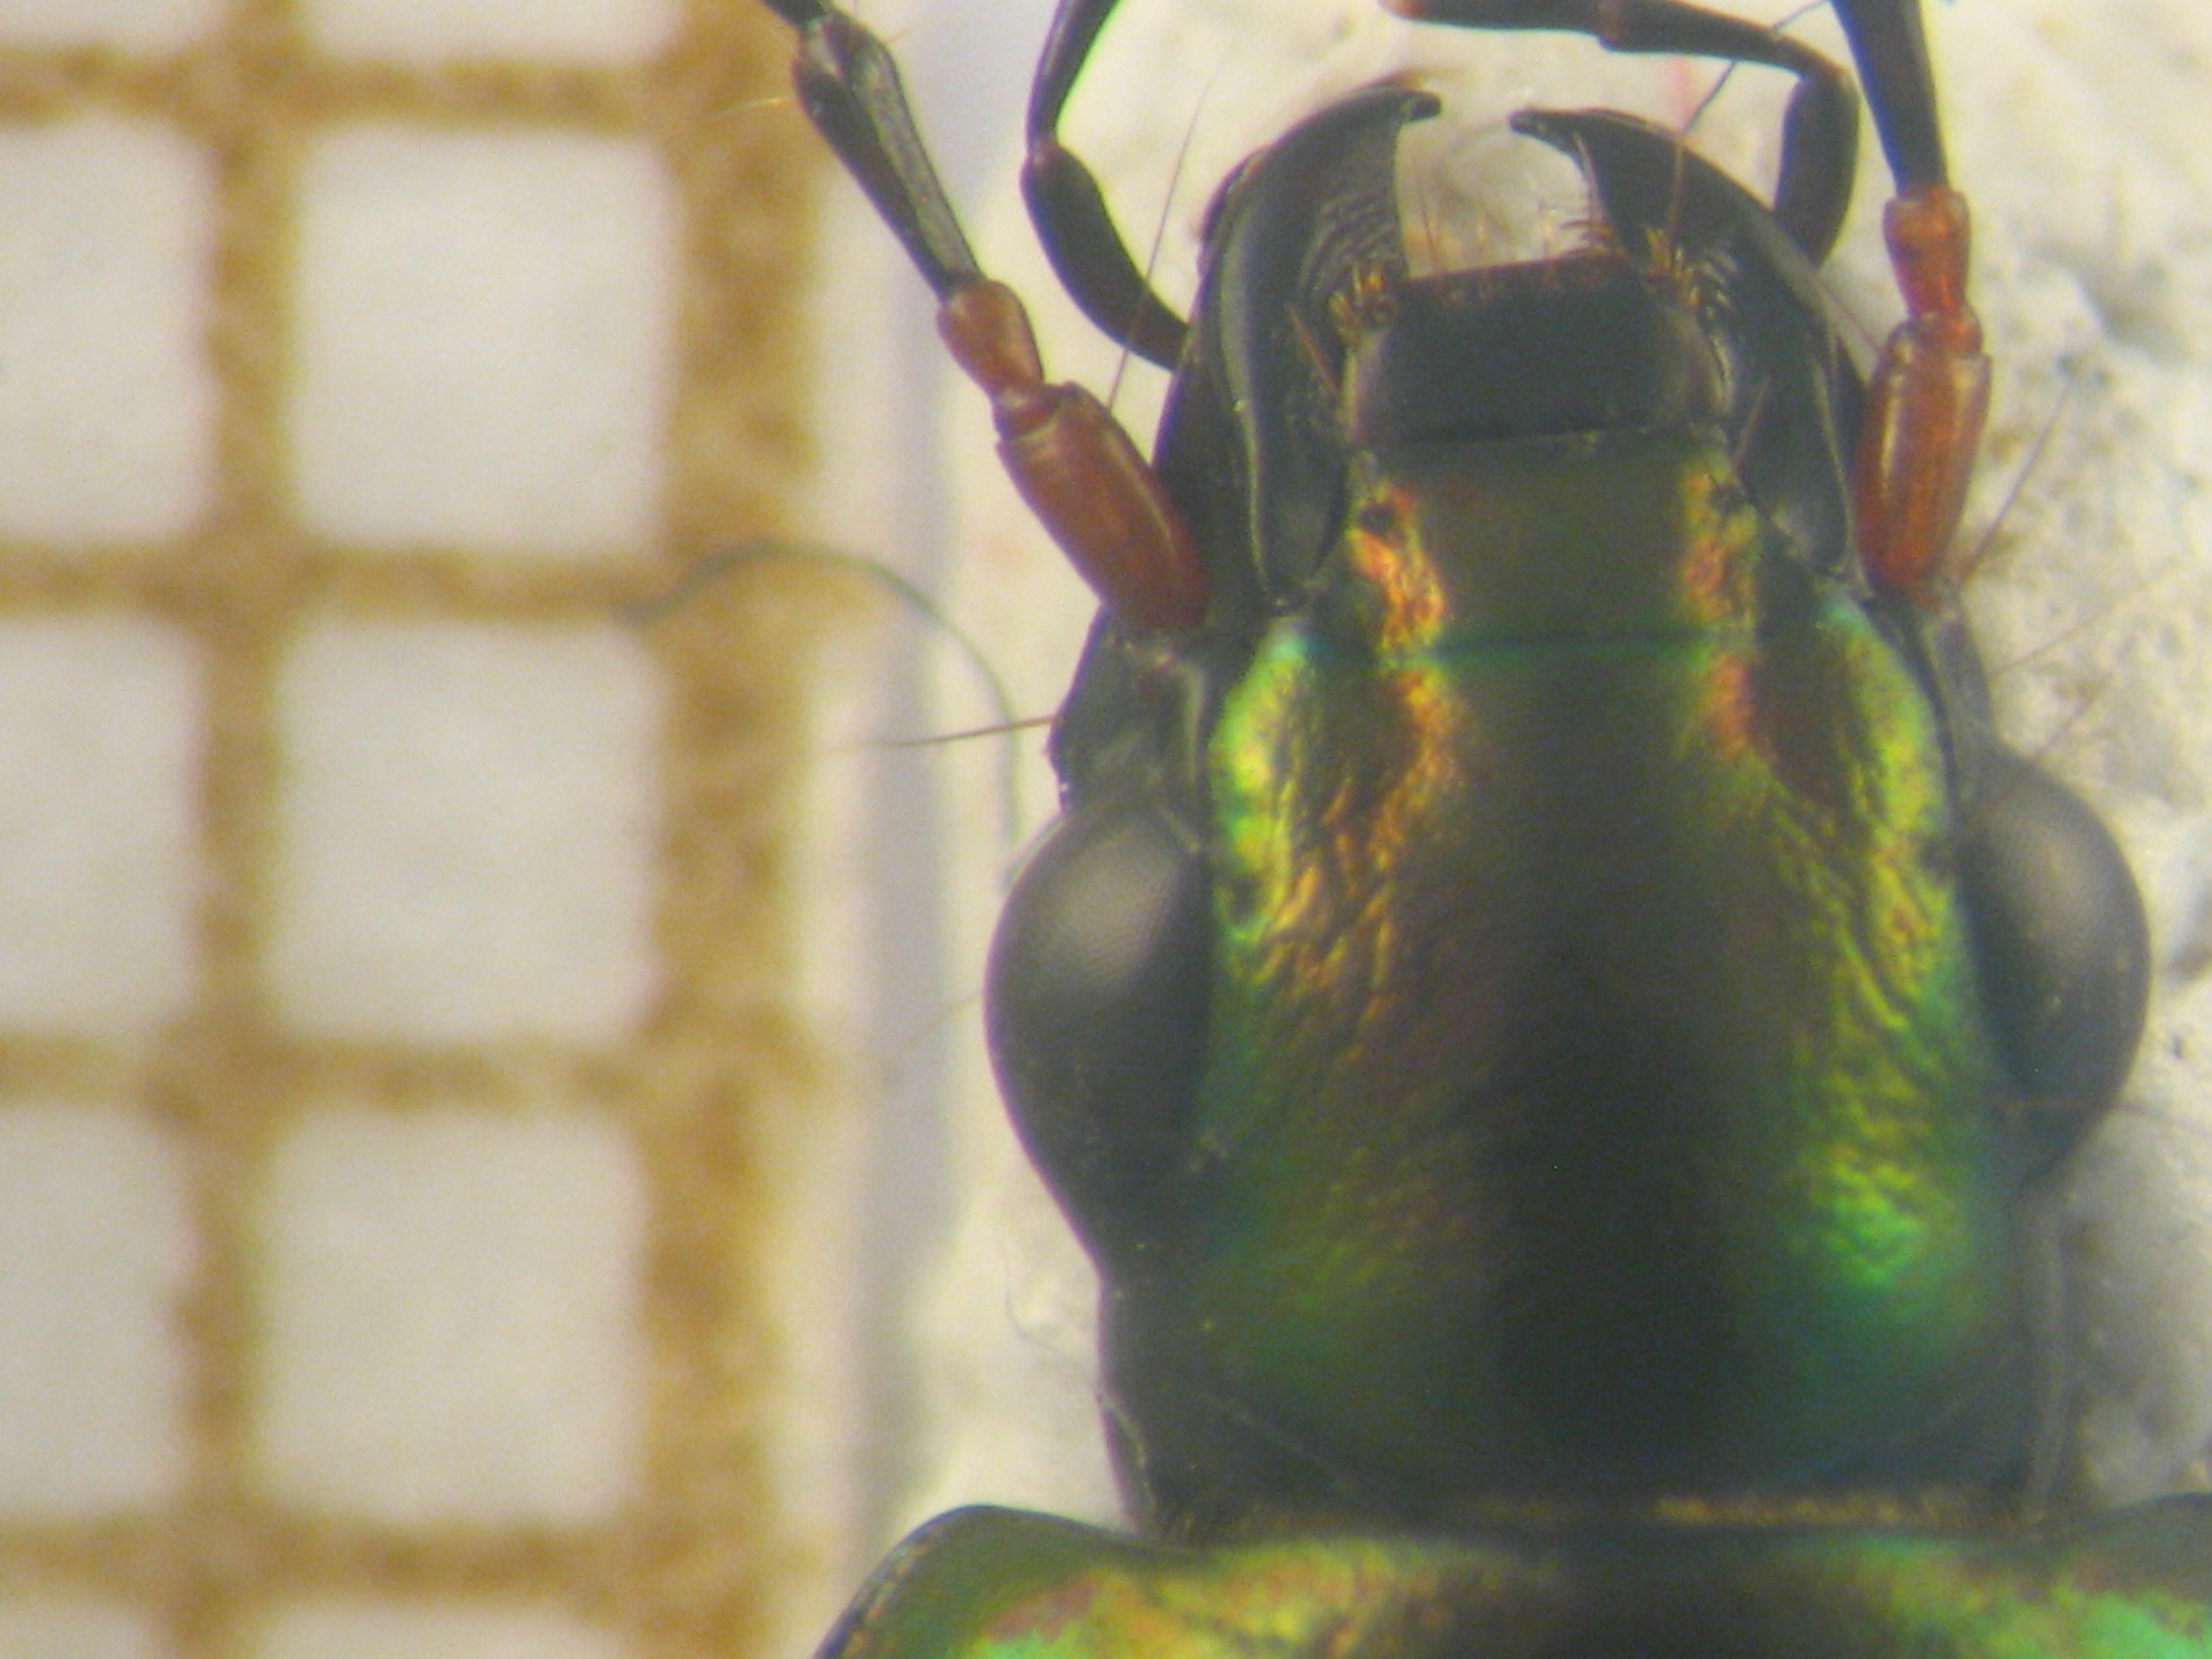
\includegraphics[width=0.22\textwidth]{./images/tete}}~~
\subfloat[b]{\label{figrbox2}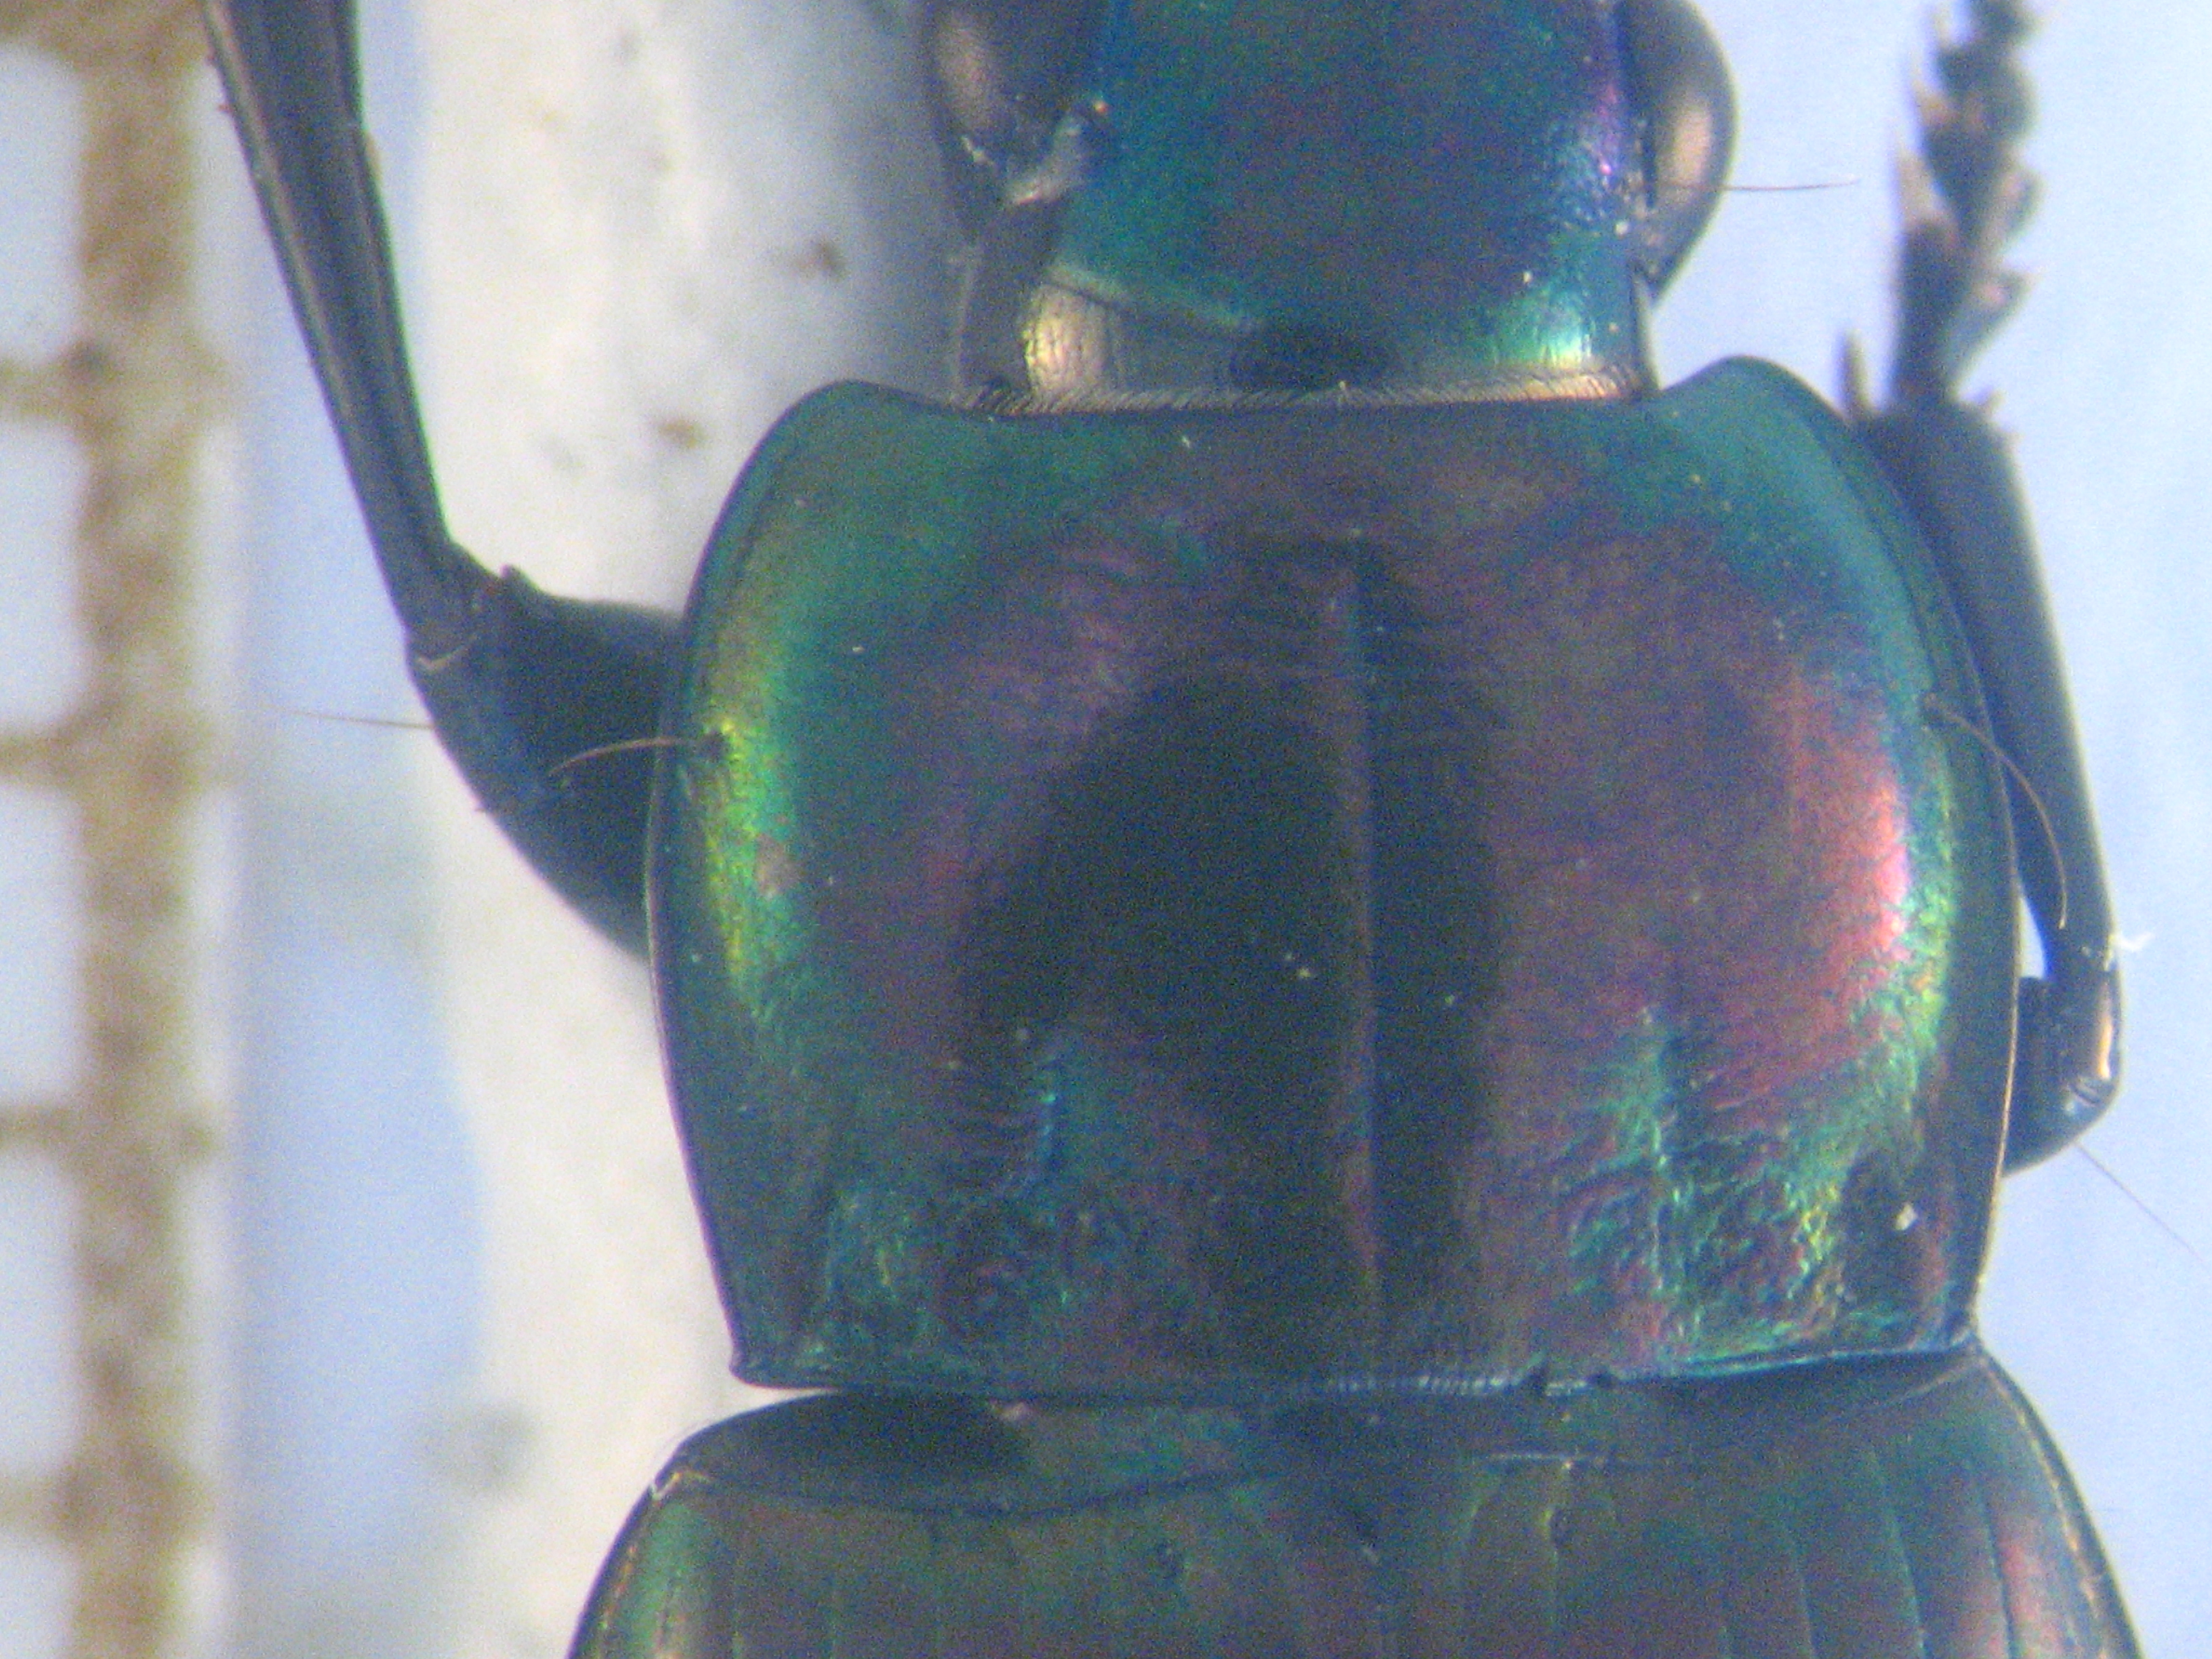
\includegraphics[width=0.22\textwidth]{./images/pronotum}}\\
\subfloat[c]{\label{figrbox1}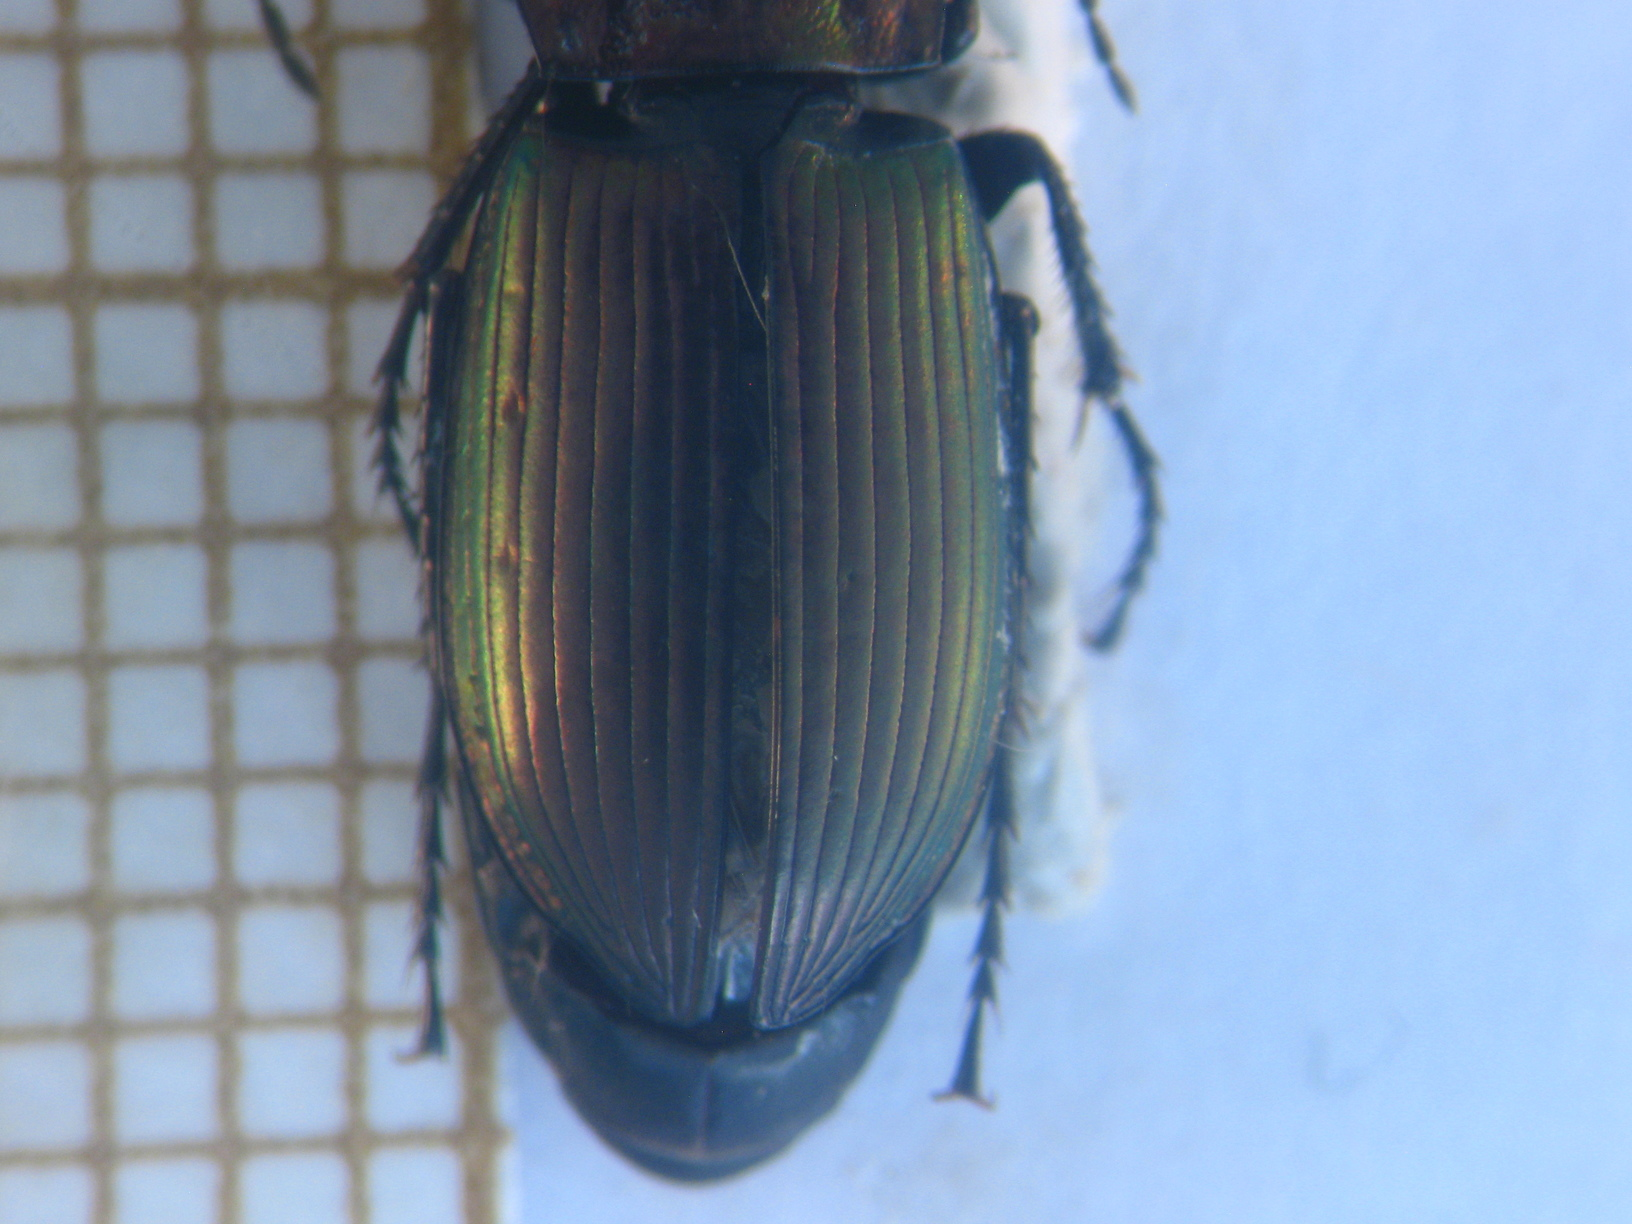
\includegraphics[width=0.22\textwidth]{./images/body}}~~
\subfloat[d]{\label{figrbox2}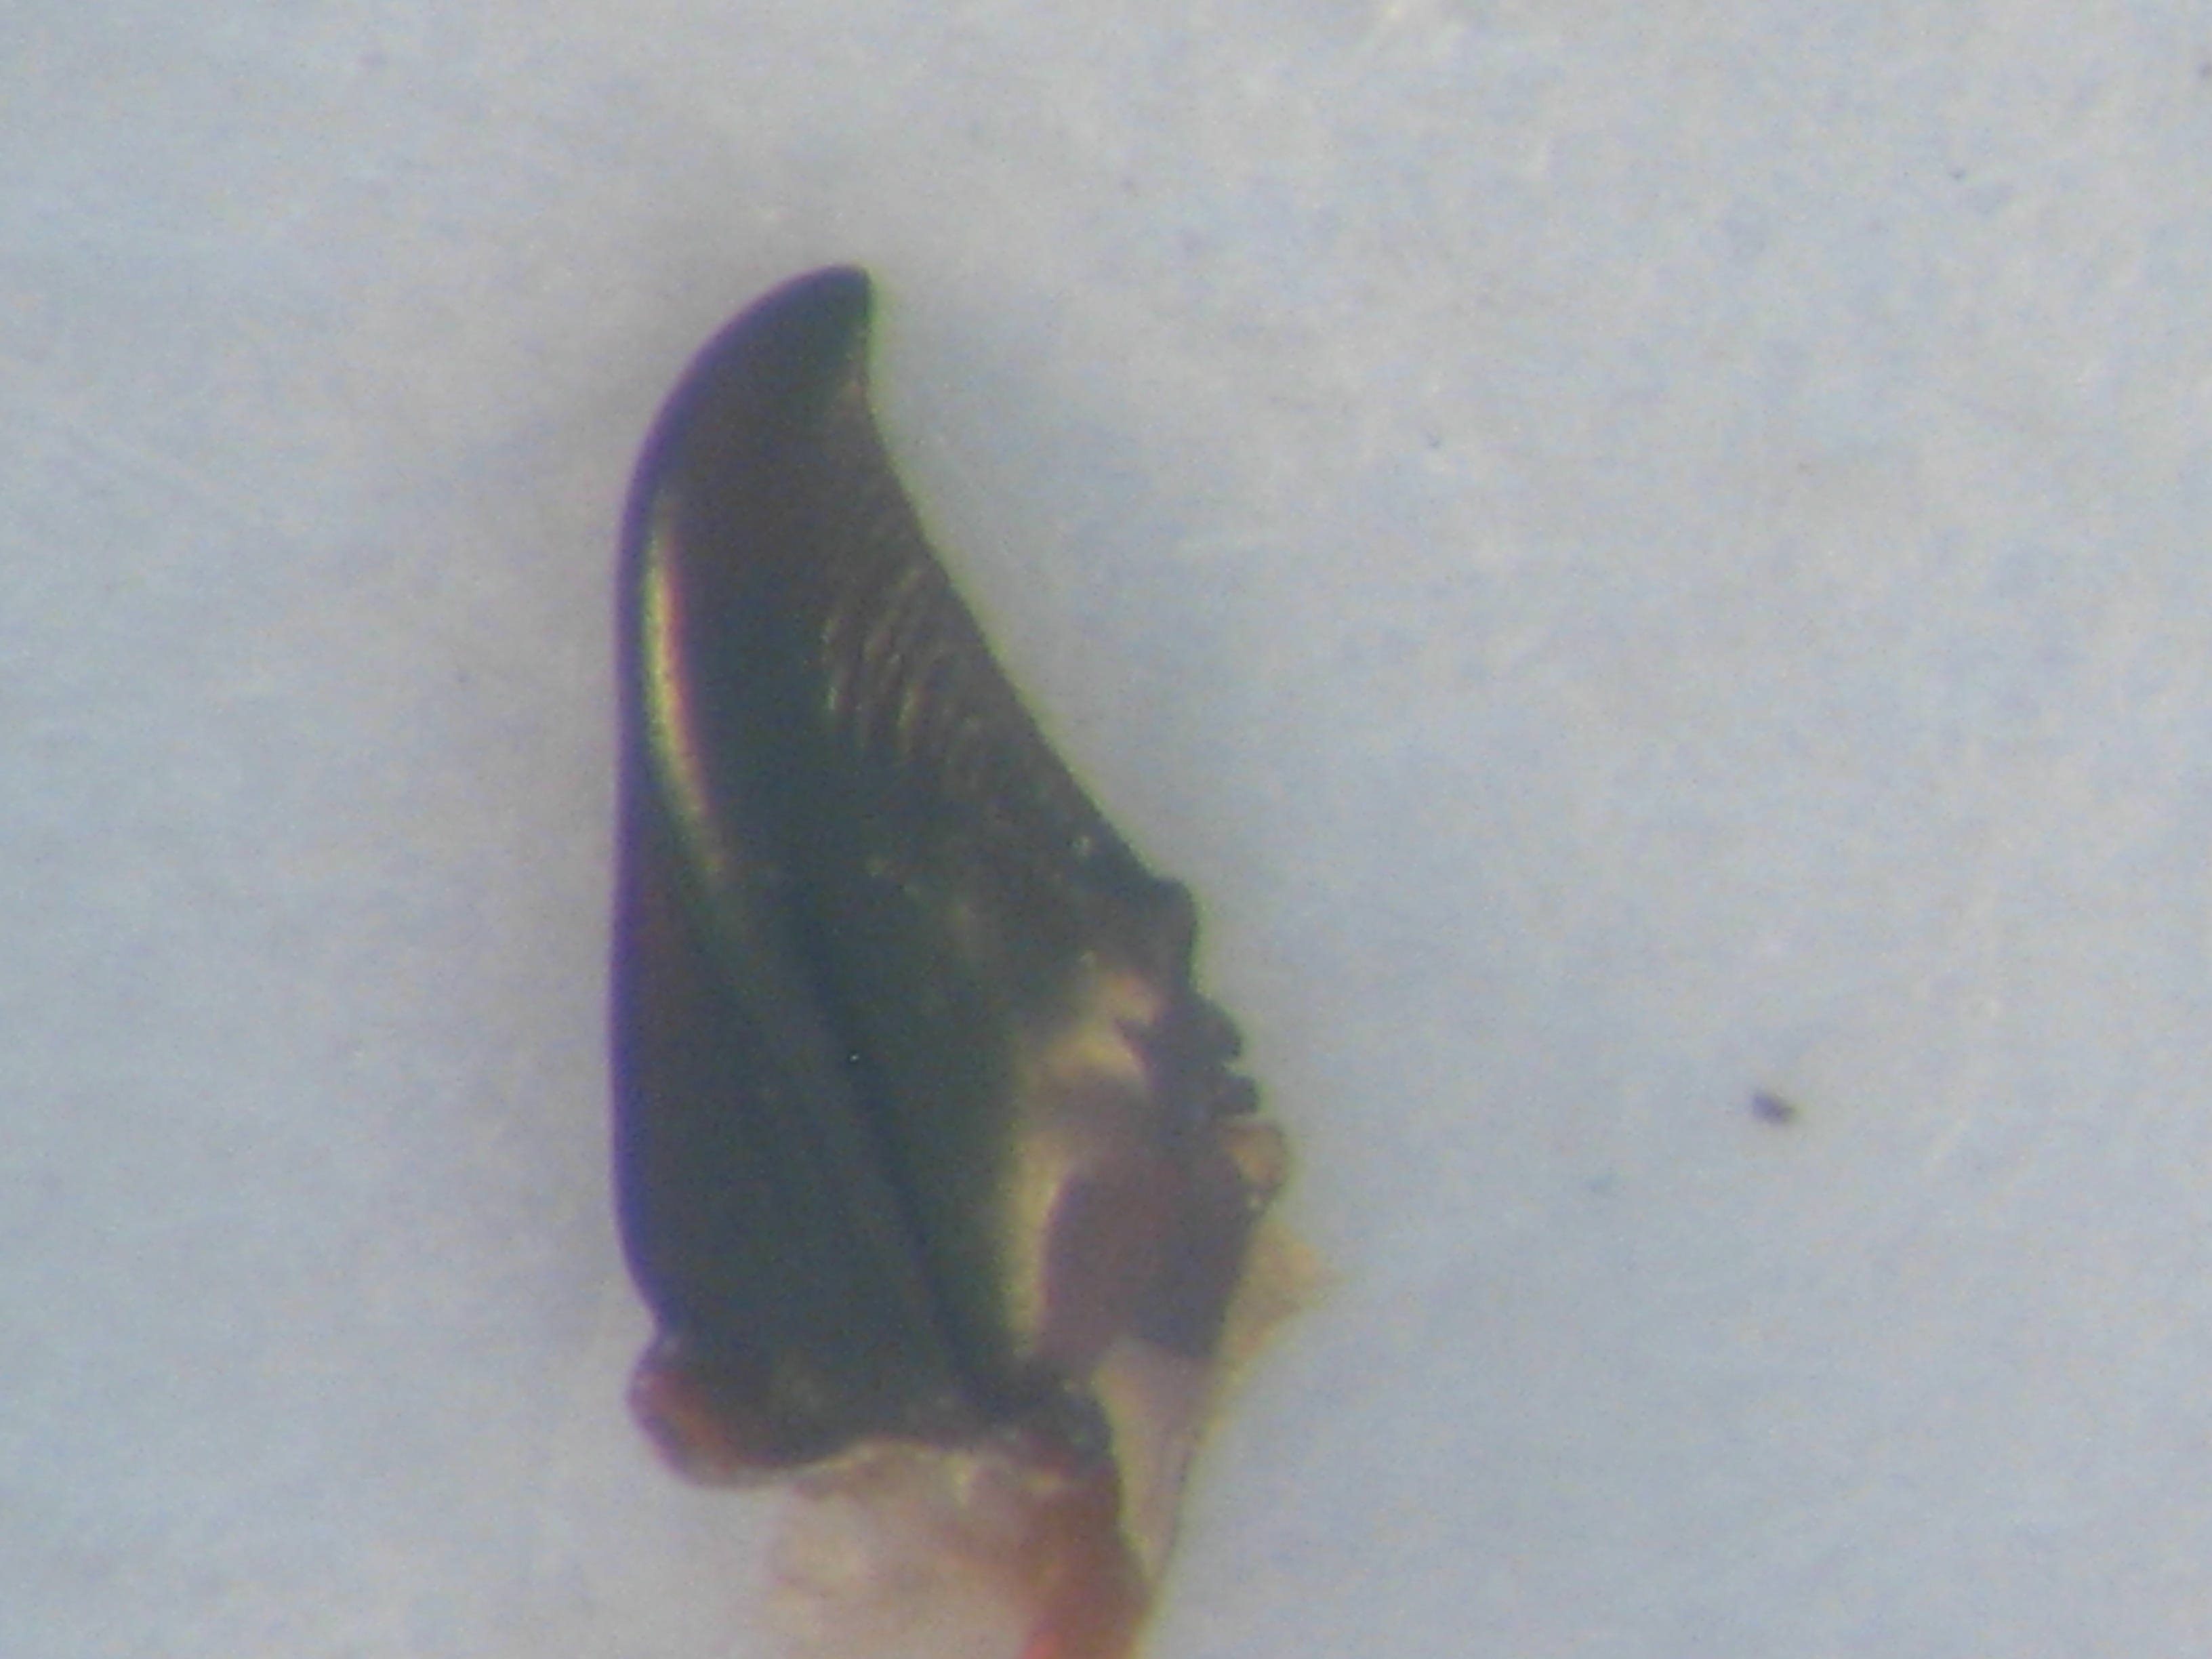
\includegraphics[width=0.22\textwidth]{./images/lm}}\\
\subfloat[e]{\label{figrbox1}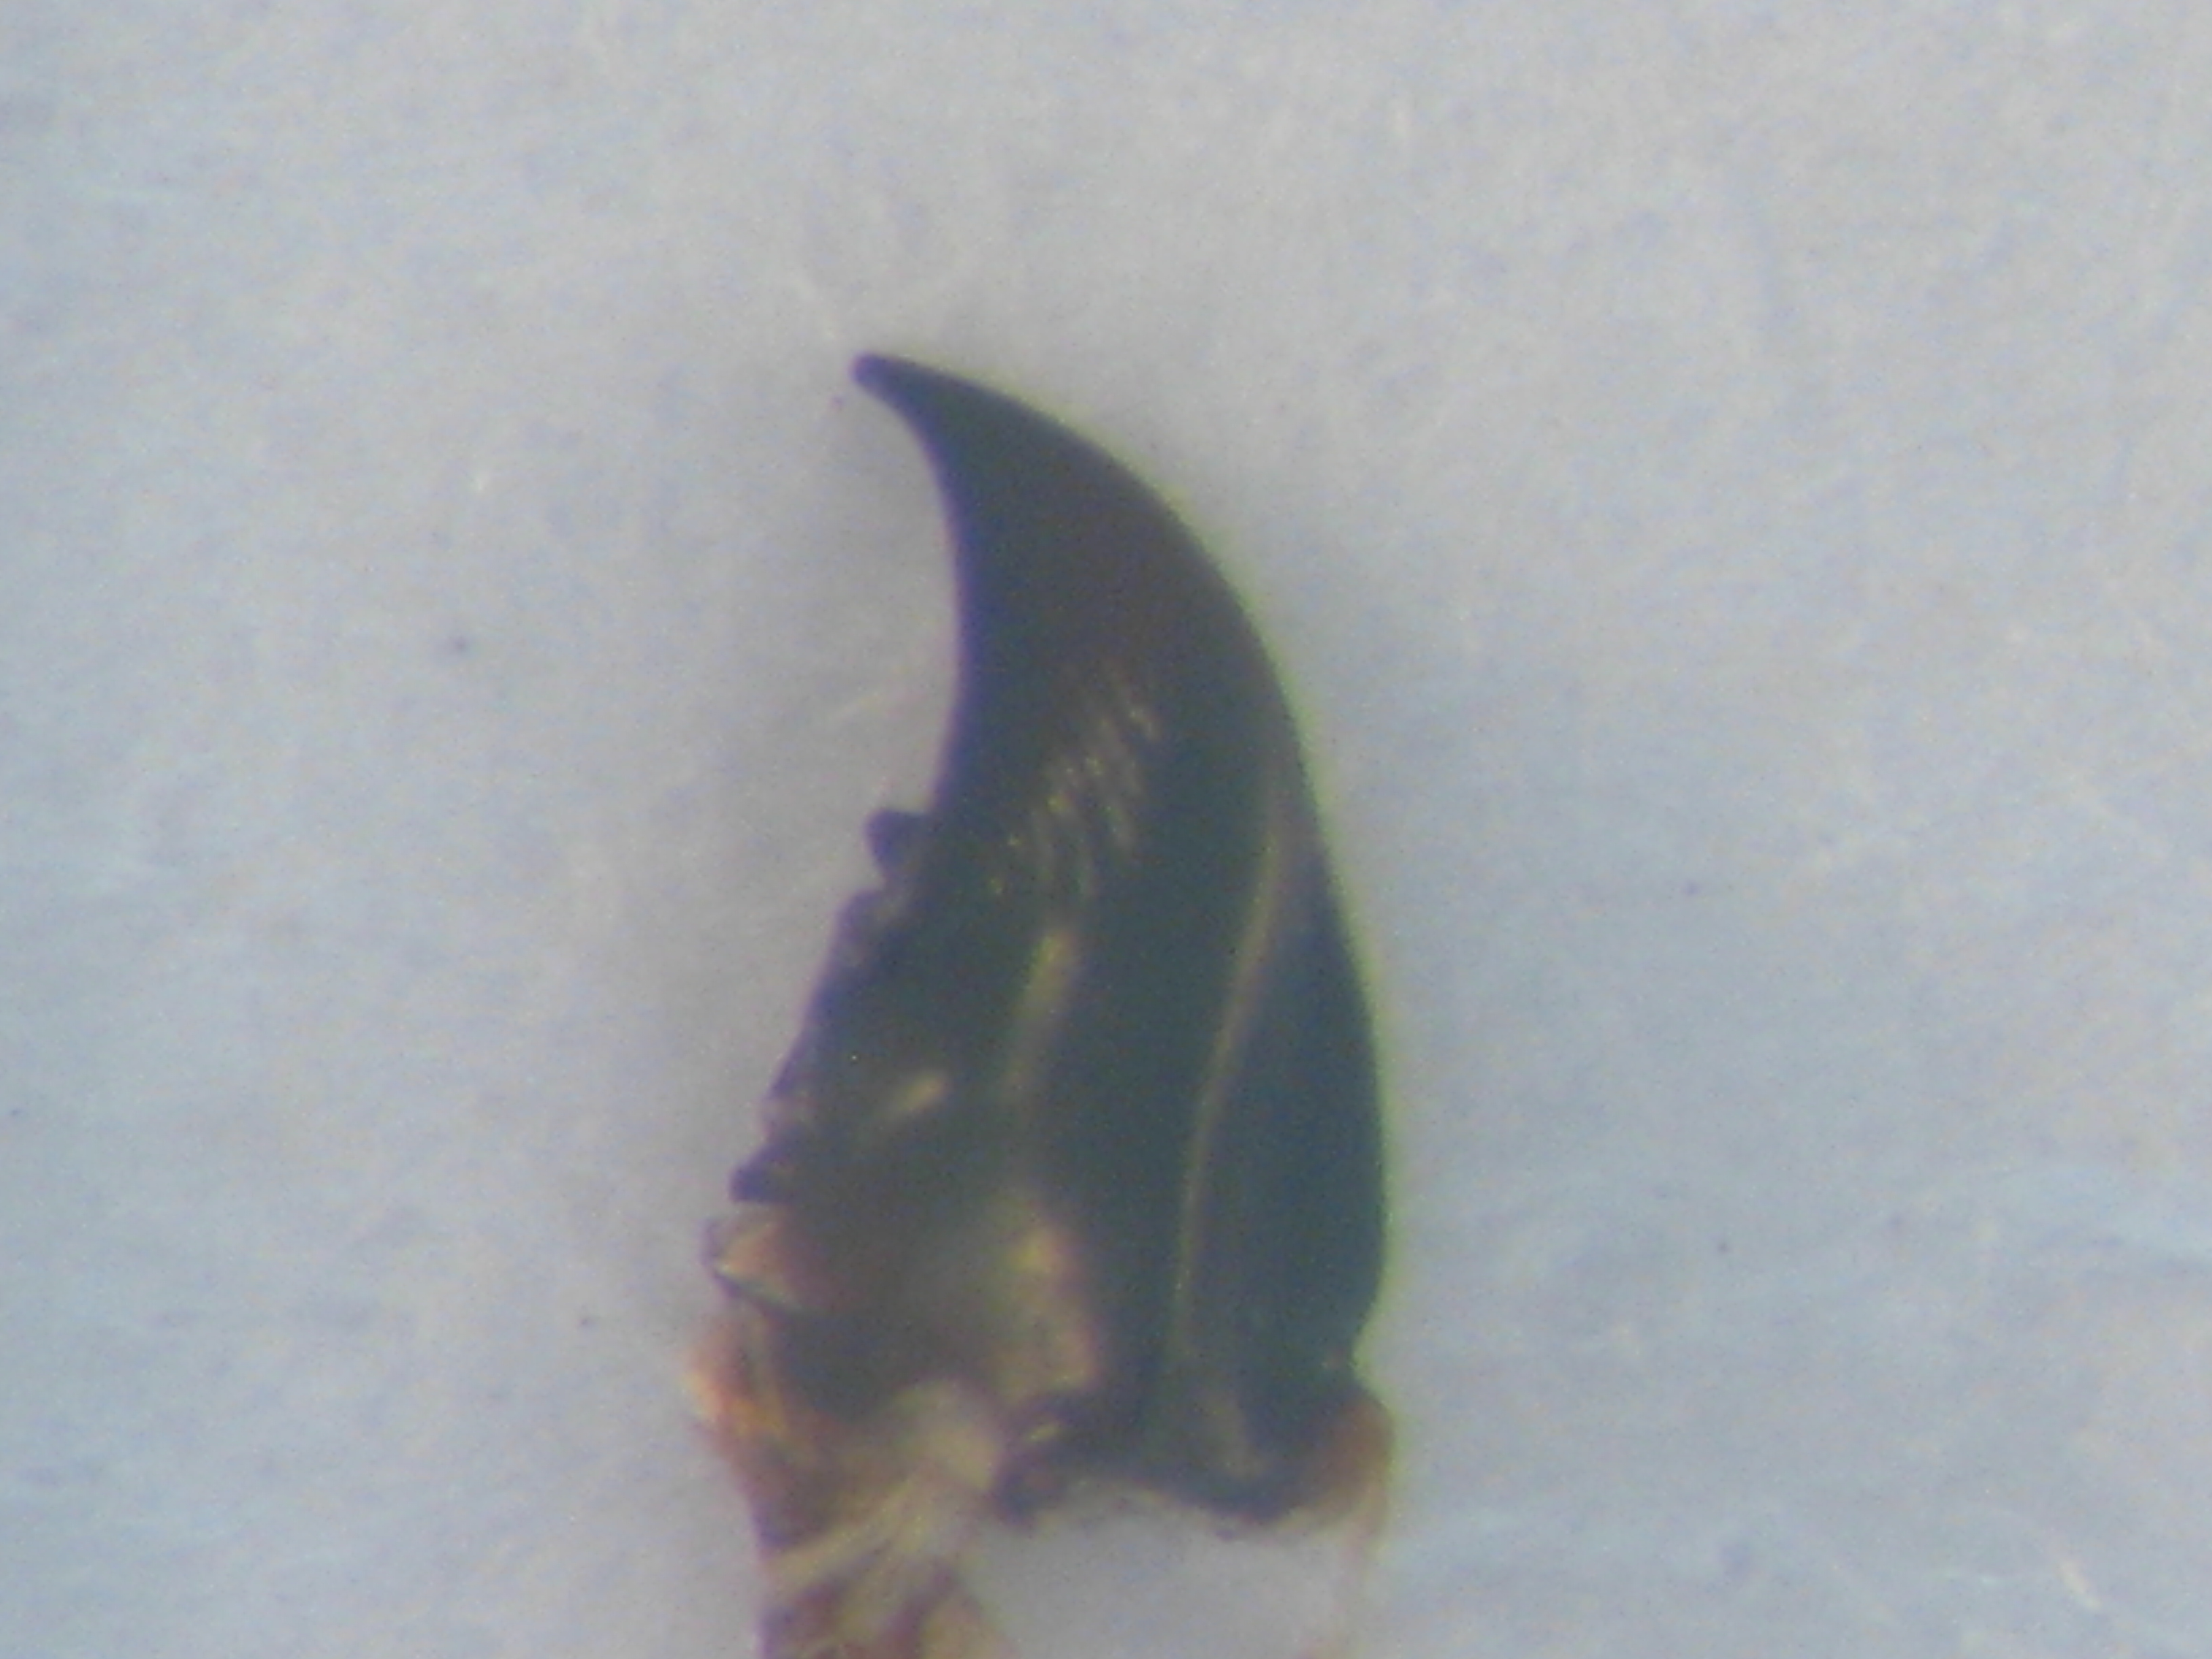
\includegraphics[width=0.22\textwidth]{./images/rm}}
\caption{The parts of beetle: (a) head, (b) pronotum, (c) body, (d,e) left and right mandible}
\label{figparts}
\end{figure}~\\[0.2cm]
In this paper, we focus on a method that can automatic idenfication of landmarks on 2D images of beetle, specify the mandibles of beetle. The method mainly includes three stages: firstly, we extract the feature of the object in the image; secondly, the automatic landmarks are indentified by image registration and generalizing Hough transform; finally, a refinement of the estimated landmarks is done by cross-correlation.\\[0.2cm]
In section 2, the steps of our methods will be discussed. All experiments and evaluation are described in section 3. Finally, we have some conclusion and discussion in the section 4.

\section{Method}
For each image, a set of manual landmarks have been set by biologists corresponding to the morphological points of interest (18 landmarks for each right mandible and 16 landmarks for each left mandible). The automatic procedure to determine the landmarks is based on the segmentation of the image. The presence between two images are indicated by generalizing Hough transform, along with theirs translation and rotation are determine by applying registration. The last step is using cross-correlation to verify the location of estimated landmarks.
\subsection{Image segmentation}
In the methods of image processing, feature extraction is always a important stage. Besides, depending on the nature of the method, the methods are applied before (pre-processing) or after (post-process) extracting the features. In our method, the original Canny alogrithm\cite{canny} is ideal for detect the curves on the image. The ratio between lower threshold and upper threshold which are used in Canny algorithm is 1:3 (lower threshold approximated to 1 times \textit{threshold value} and upper threshold set to 3 times threshold value). This value is evaluated by the experiments. The \textit{threshold value} has been determined by analyzing the image histogram. During appling the Canny alogrithm to detect the curves of object, the gradient direction of each pixel which belongs to the curves is kept for the next step of the method. 
\begin{figure}[h]
\centering
\subfloat[Segmentation result after applying Canny algorithm]{\label{figrbox1}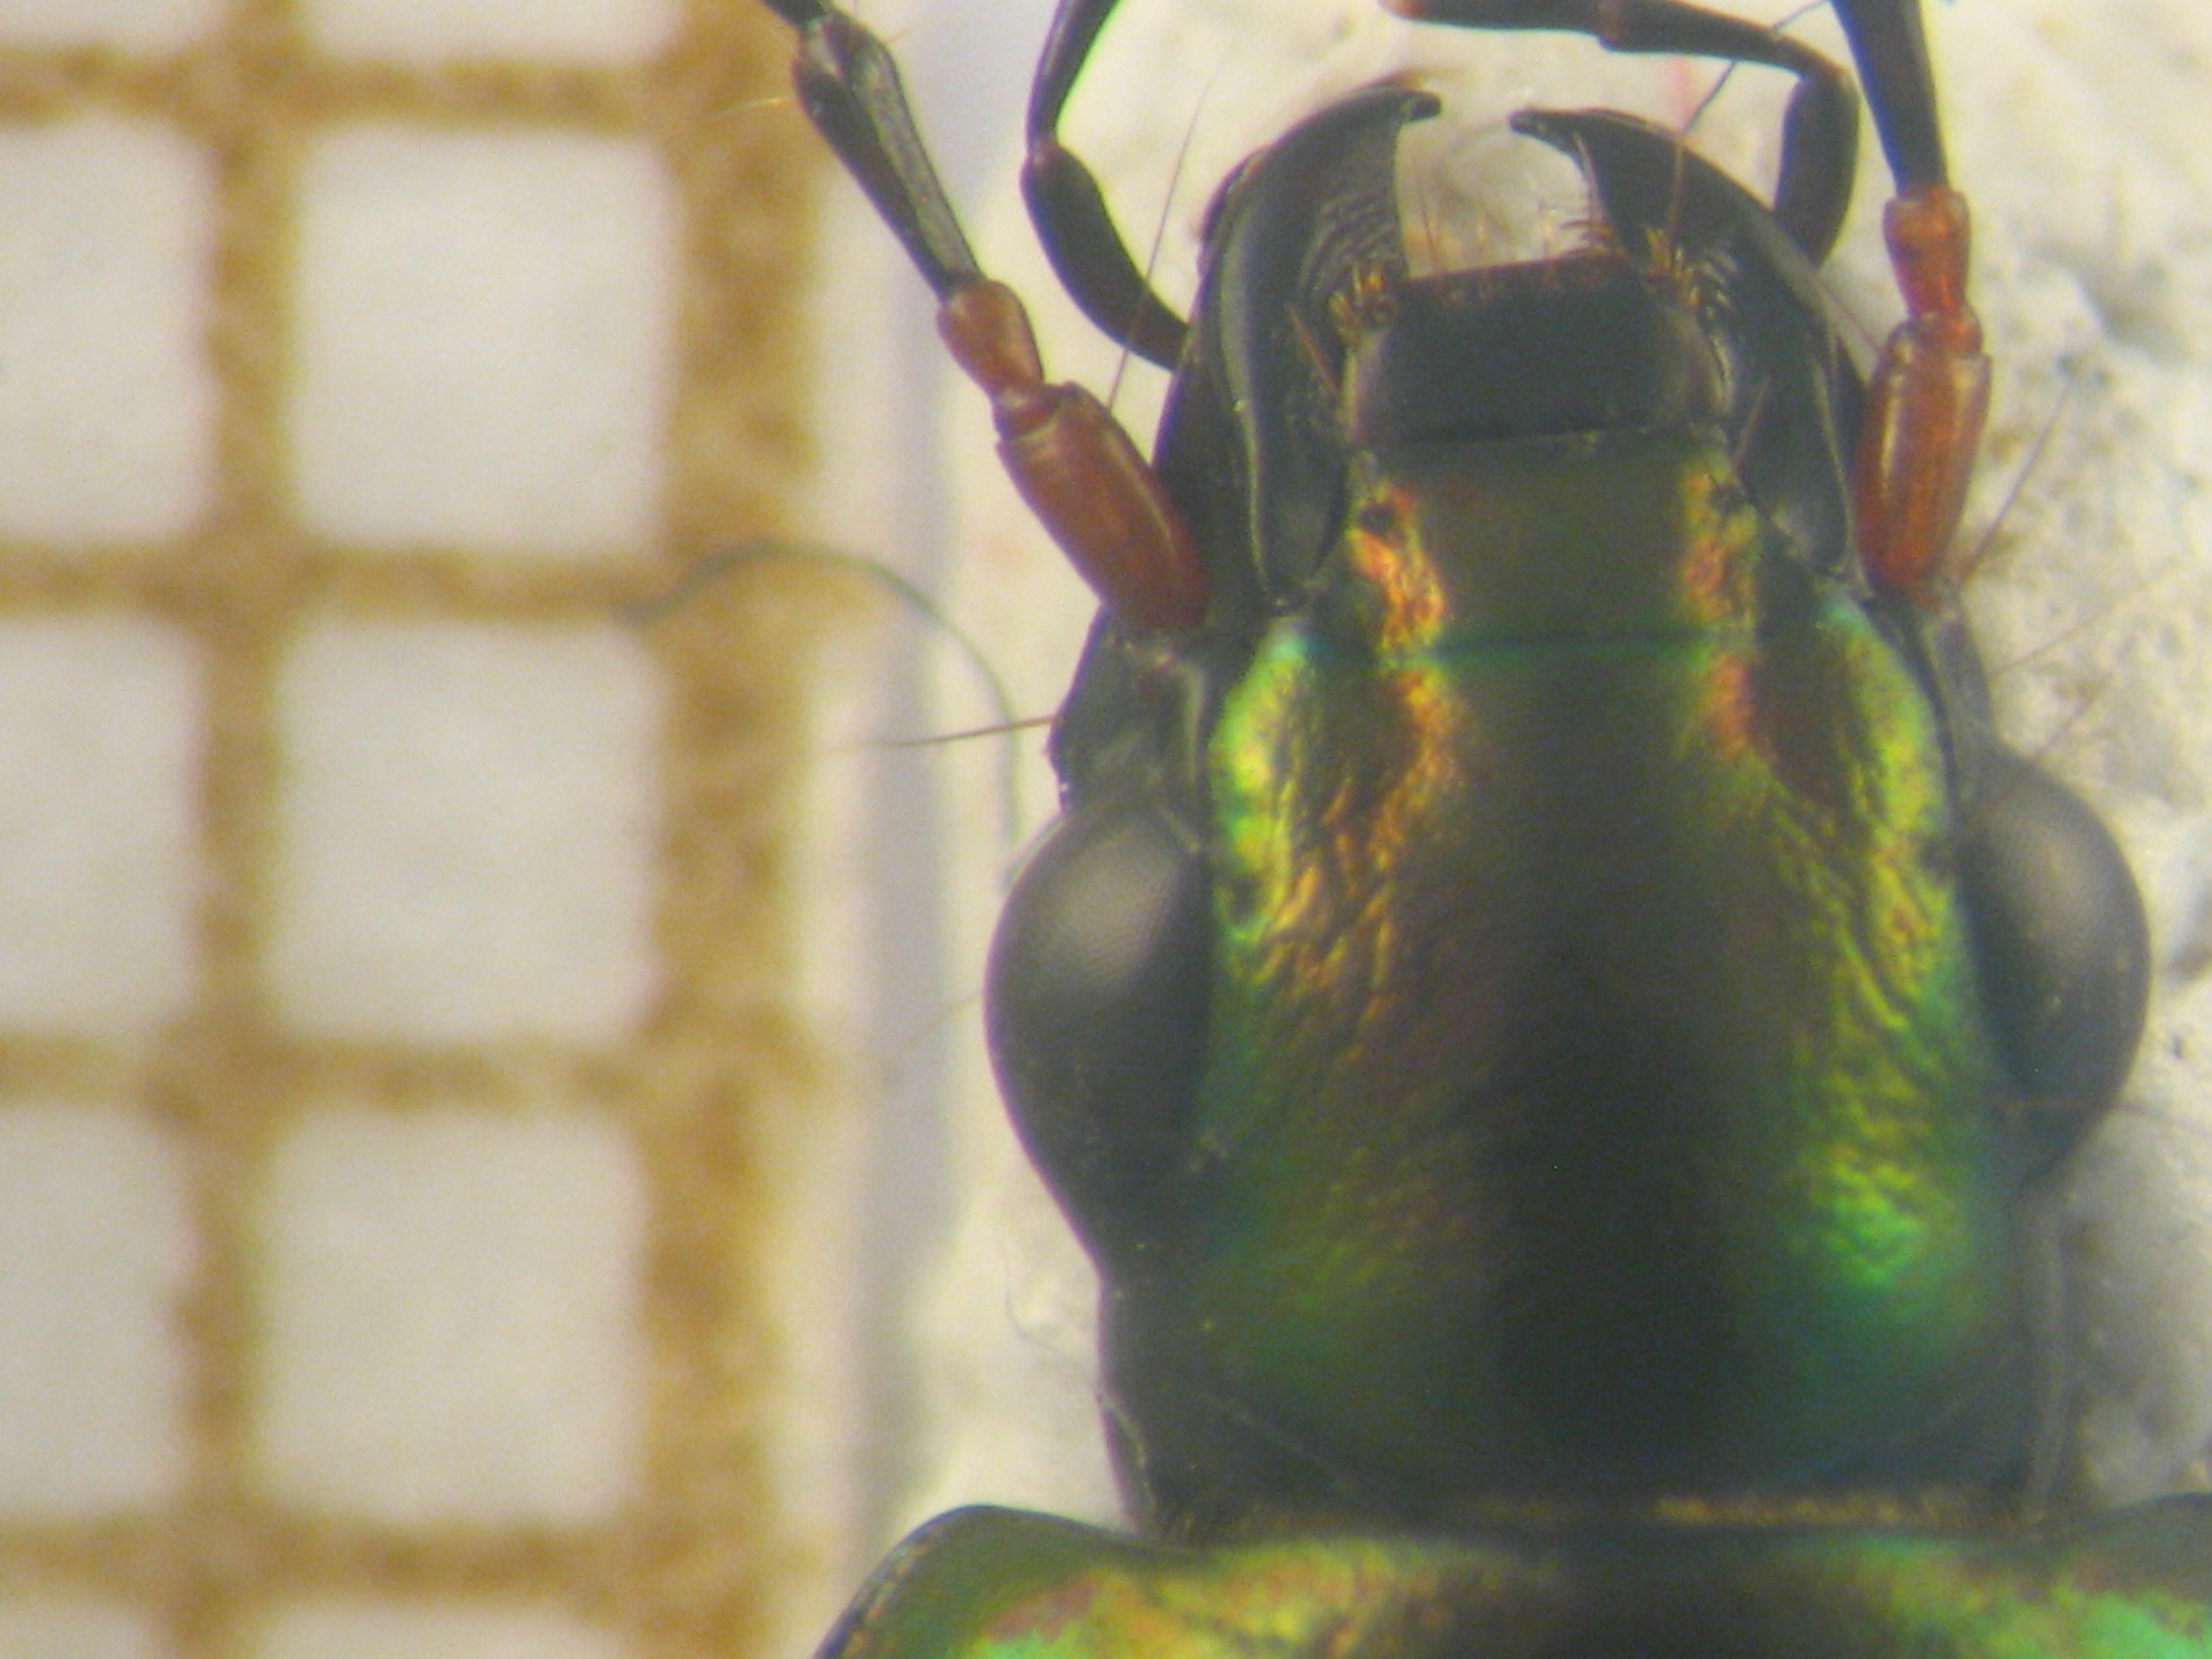
\includegraphics[width=0.22\textwidth]{./images/tete}}~~
\subfloat[Segmentation result after applying Canny algorithm and post-process]{\label{figrbox2}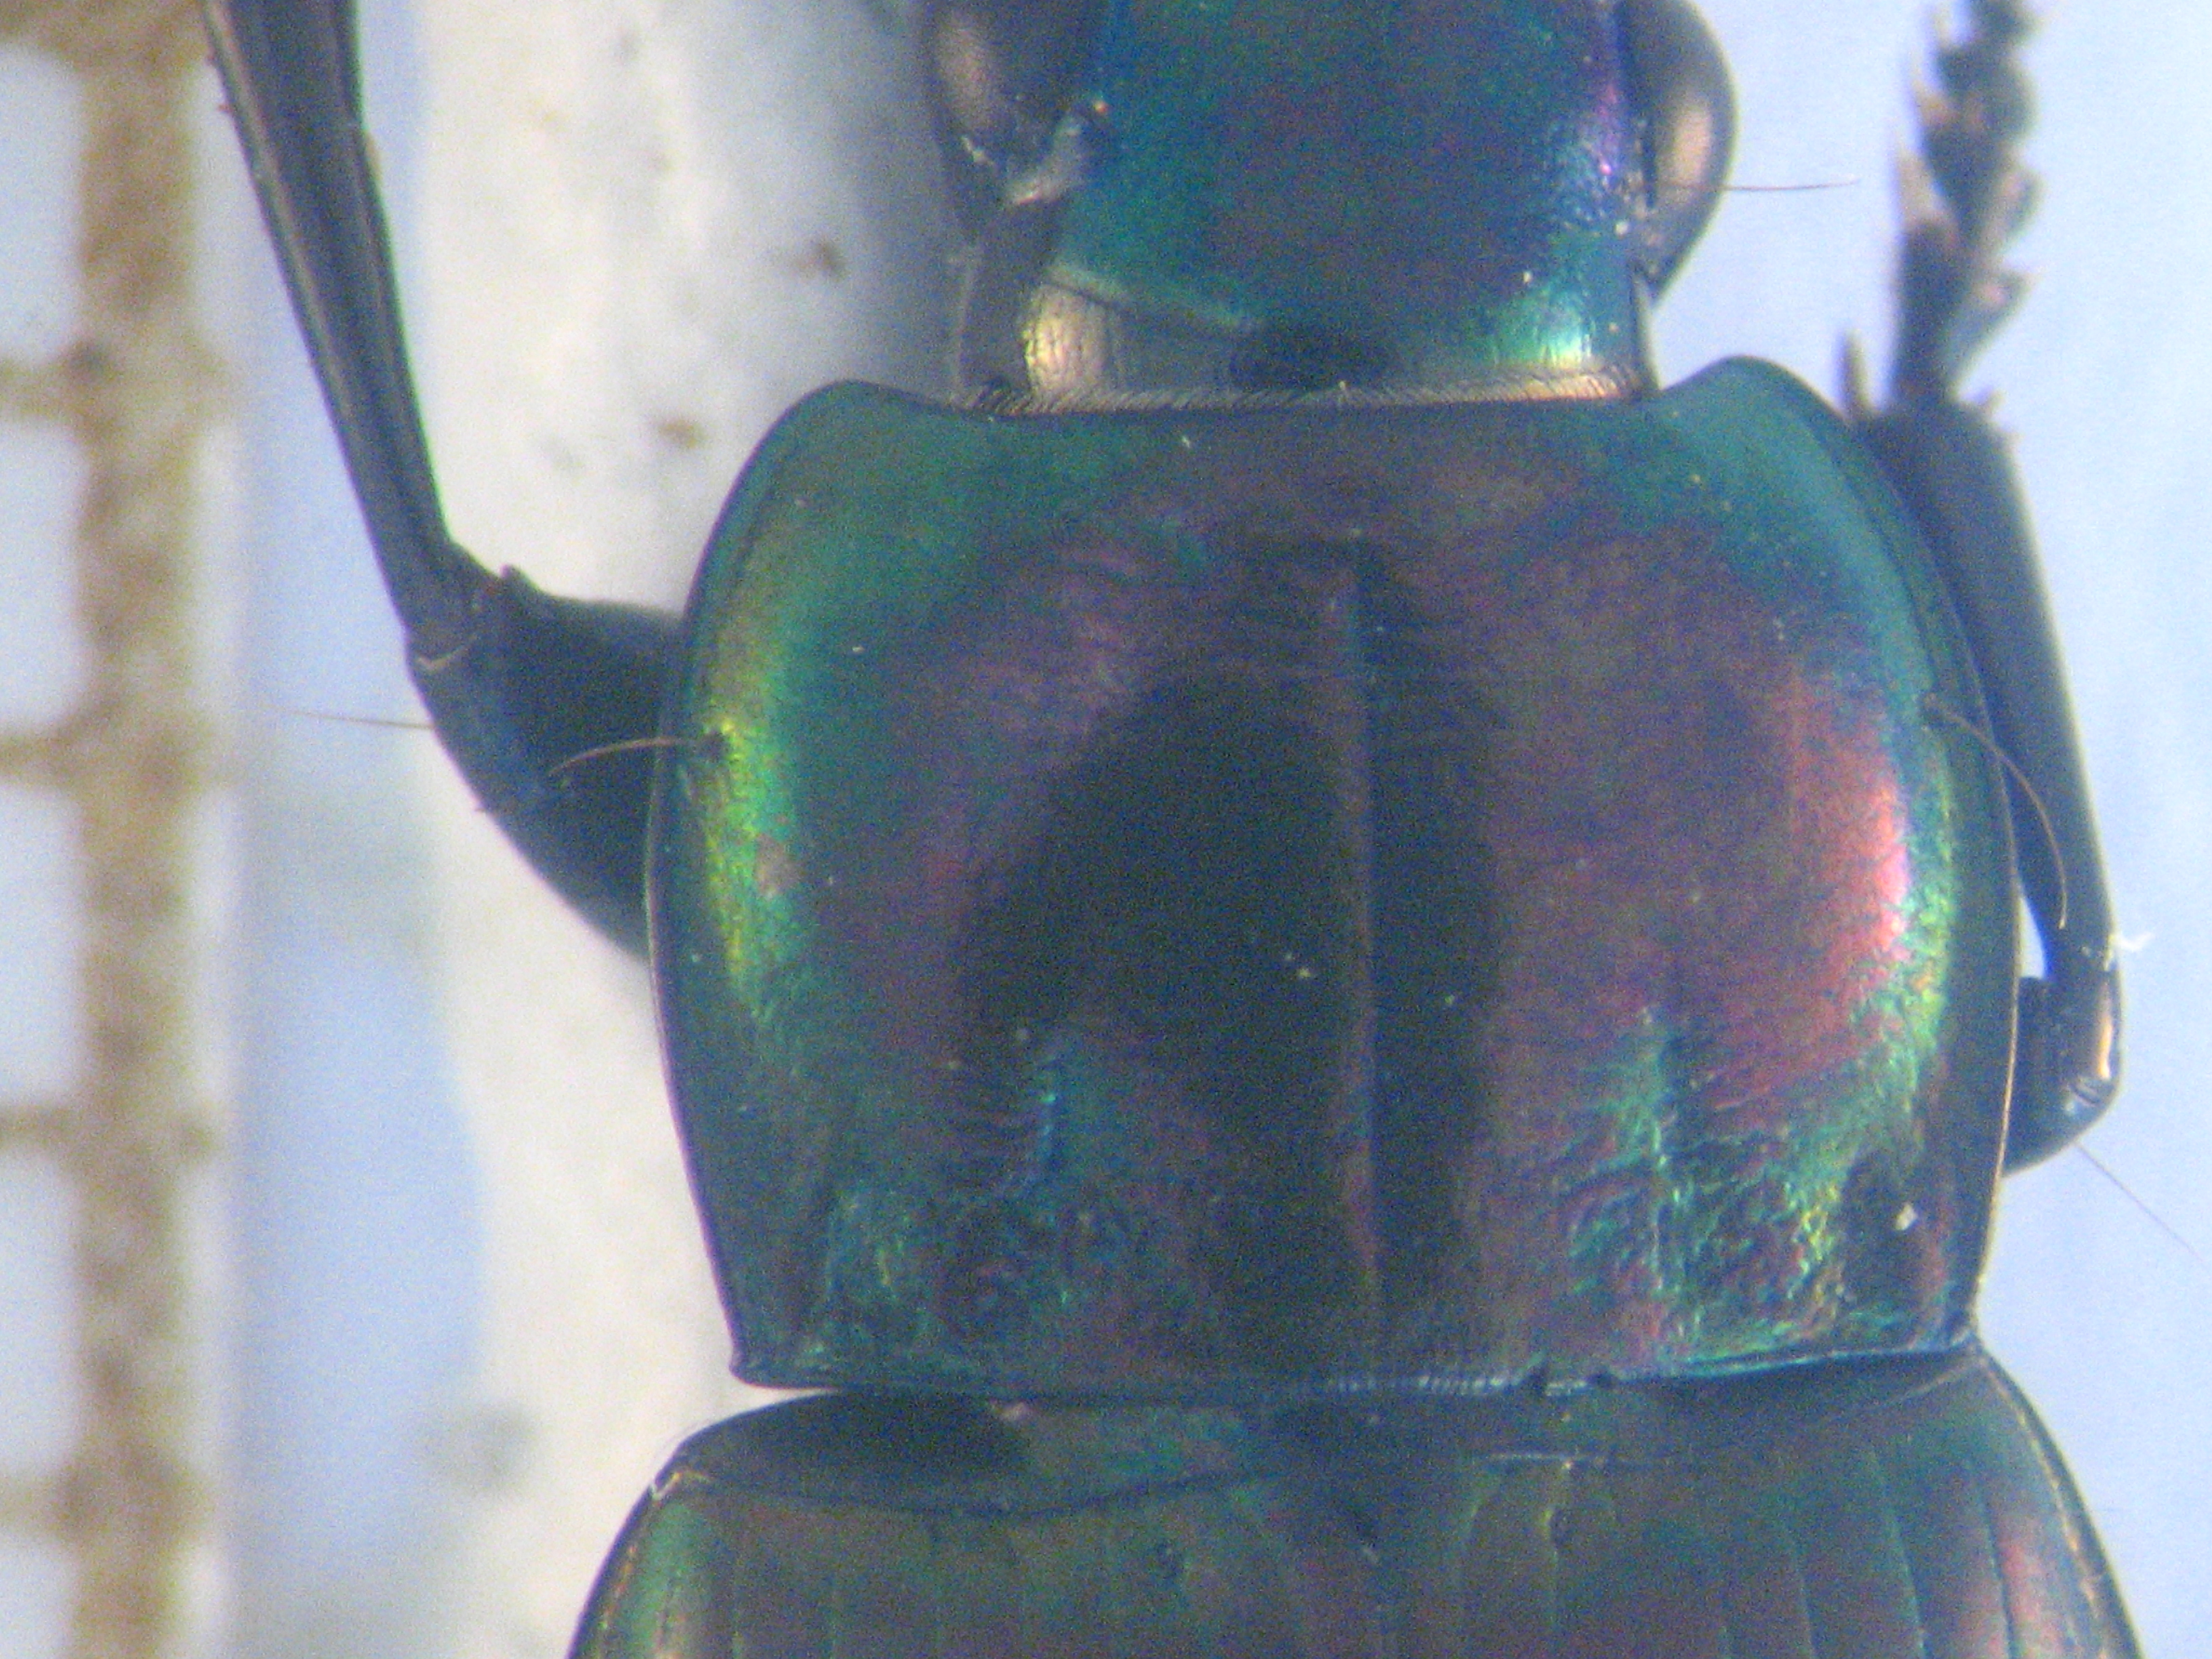
\includegraphics[width=0.22\textwidth]{./images/pronotum}}
\caption{The segmentation results of the image}
\label{figparts}
\end{figure}~\\[0.2cm]
In this study, the aim of segmentation stage is determined the outer border of the object which can be used to reconstruct the shape of the object as well as provide the best data for next step. The curves from Canny algorithm will be post-processed to remove the unnecessary curves i.e hole inside the border. 
\subsection{Generalizing Hough transform}
The generalizing Hought transform (GHT)\cite{Ballard} is a key of this study. With two input images, GHT is used to recognize the similar between two images and estimate the landmarks of an image based on the landmarks of other image. The GHT includes two phase learning and recognition process. In the learning phase of GHT, model image is used to construct R-table. This is table that contains the polar value of each point in model's curves. A polar coordinate system is initialized in the model image by fixing a reference point and using it as orgin. The R-table records the polar coordinate values of all boundary points. The rows of R-table are indexed by the gradient directons of the points on the curves. It means that with a gradient direction can be exists many polar coordinate values. During the recognition phase, a 2D accumulator is used, called Hough Space Voting (HSV). The axes of HSV express the information of polar coordinate system. For each curve points on scene image, we try to find a record in R-table that corresponding with the gradient direction of each scene point. The voting will be carried out at all location in HSV that found in R-table. At the end of voting process, if the scene image is identical to the model image, then the cell where have the highest number of votes corresponds to the reference point of the model in the scene image. Besides, the peak value would be equal to the number of curve points of the scene image when the model and scene image match perfectly.
\section{Typeset text}
\subsection*{Normal or Body Text}
Please use a 10-point Times Roman font, or other Roman font with serifs, as close as possible in appearance to Times Roman in which these guidelines have been set. The goal is to have a 10-point text, as you see here. Please use sans-serif or non-proportional fonts only for special purposes, such as distinguishing source code text. If Times Roman is not available, try the font named Computer Modern Roman. On a Macintosh, use the font named Times.  Right margins should be justified, not ragged.

\subsection*{Title and Authors}
The title (Helvetica 18-point bold), authors' names (Helvetica 10-point) and affiliations (Helvetica 10 point) run across the full width of the page -- one column wide. We also recommend e-mail address (Helvetica 10 point). See the top of this page for three addresses. If only one address is needed, center all address text. For two addresses, use two centered tabs, and so on. For more than three authors, you may have to improvise.\footnote{If necessary, you may place some address information in a footnote, or in a named section at the end of your paper, but margins must remain empty.} 

\subsection*{First Page Copyright Notice}
Please include 3.8 cm (1.5") text box with the text shown at the bottom of the left column of the first page with the copyright notice.

\subsection*{Others Pages}
Others pages start at the top of the page (margin 2.5 cm) and continue in double-column format.  The two columns on the last even page should be as close to equal length as possible. 

{\bfseries Total length of a paper is max. 8 pages.}

Footnotes should be Times New Roman 9-point, and justified to the full width of the column.

Please, use the standard Journal of WSCG format for references -- that is, a numbered list at the end of the article, ordered alphabetically by first author, and referenced by a name in brackets \cite{con00a}. See the examples of citations at the end of this document. Within this template file, use the style named references for the text of your citation.

The references are also in 9 pt., but that section (see Section \ref{references}) is ragged right. References should be published materials accessible to the public. Internal technical reports may be cited only if they are easily accessible (i.e. you can give the address to obtain the report within your citation) and may be obtained by any reader. Proprietary information may not be cited. Private communications should be acknowledged, not referenced, e.g. "[Adam, personal communication]").

\subsection*{Page Numbering, Headers and Footers}
Do not include headers, footers or page numbers in your submission. These will be added when the publications are assembled.

\begin{figure}[htb]
    \centering
    \rule{6cm}{3cm}
    \caption{Insert caption to place caption below figure.}
    \label{fig:box}
\end{figure}

\begin{table}[htb]
	\centering
	\begin{tabular}{|l|l|l|l|}
	\hline
	Graphics & Top & In-between & Bottom \\
	\hline
	Tables & End & Last & First \\
	\hline
	Figures & Good & Similar & Very well \\
	\hline
	\end{tabular}
	\caption{Table captions should be placed below the table}
\end{table}

\section{Figures/Captions}
Place Tables/Figures/Images in text as close to the reference as possible (see Fig.\ref{fig:box}). It may extend across both columns to a maximum width of 16 cm (6.3"). Captions should be Times New Roman 10-points.  They should be numbered (e.g., "Table 1" or "Figure 2"), please note that the word for Table and Figure are spelled out. Figure's and Table's captions should be centered beneath the image, picture or a table.

\section{Sections}
The heading of a section should be in Times New Roman 12-point bold in all-capitals flush left with an additional 6-points of white space above the section head.  Sections and subsequent sub- sections should be numbered and flush left. For a section head and a subsection head together (such as Section 3 and Subsection 3.1), use no additional space above the subsection head.

\subsection{Subsections}
The heading of subsections should be in Times New Roman 12-point bold with only the initial letters capitalized. (Note: For subsections and subsubsections, a word like the or a is not capitalized unless it is the first word of the header.)

\subsubsection{Subsubsections}
The heading for subsubsections should be in Times New Roman 11-point italic with initial letters capitalized and 6-points of white space above the subsubsection head.

\section{Acknowledgments}
Our thanks to ACM SIGCHI and SIGGRAPH for allowing us to modify templates they had developed.

%-------------------------------------------------------------------------
% example of algorithm typesetting
% to allow this, uncomment line 
% \RequirePackage[noend]{myalgorithm}
% in the wscg.sty file
% and download that package from Gabriel Zachmann's page http://zach.in.tu-clausthal.de/latex/
%
%
%\begin{algorithm}
%\hrule
%  \centering
%\begin{algorithmic}
%    \STMT $d_{l,r} = f_B(P_1), f_B(P_n)$
%    \WHILE{ $|d_l| > \epsilon $ and $|d_r| > \epsilon $ and $l<r$}
%        \STMT $d_x = f_B(P_x)$
%        \IF{ $d_x < 0$ }
%            \STMT $l, r = x, r$
%        \ELSE
%            \STMT $l, r = l, x$
%        \ENDIF
%    \ENDWHILE
%\end{algorithmic}
%\hrule
%\caption{Example of some pseudo-code}
%\label{fg:code}
%\end{algorithm}


%-------------------------------------------------------------------------

\begin{thebibliography}{99}
\label{references}
\bibitem[1]{canny} Canny, John. "A computational approach to edge detection." IEEE Transactions on pattern analysis and machine intelligence 6 (1986): 679-698.
\bibitem[2]{Ballard} Ballard, Dana H. "Generalizing the Hough transform to detect arbitrary shapes." Pattern recognition 13.2 (1981): 111-122.
\bibitem[Con00b]{con00b} Mackay, W.E. Ethics, lies and videotape, in Conf.proc. CHI'00, Denver CO, ACM Press, pp.138-145, 2000.
\bibitem[Jou01a]{jou01a} Journal of WSCG \& WSCG templates: http://wscg.zcu.cz/jwscg/template.doc (MSWord)
http://wscg.zcu.cz/jwscg/template.pdf (PDF)
\end{thebibliography}

{\bfseries
Last page should be fully used by text, figures etc. Do not leave empty space, please. 

Do not lock the PDF -- additional text and info will be inserted, i.e. ISSN/ISBN etc. 
}


\end{document}
